\section{The Inspiration}

\frame
{
	\begin{center}
		\LARGE The Inspiration: Mimicry
	\end{center}
}

\frame
{
	\frametitle{The Inspiration: Mimicry}
	\framesubtitle{History}
	
	\begin{itemize}
		\item Henry W. Bates first published in 1862.
		\item \textbf{Content:} Similarity and dissimilarity between Heliconiinae and Ithomiinae butterflies. 
		\item Bates collected 94 species of butterfly.
		\item They were grouped according to their similar appearance.
		\item \textbf{Discovery:} Similar appearing butterfly with morphological feature pointing to different species.
		\item 67 of the 94 are classified as Ithomiinae.
		\item 27 are Heliconiinae.
	\end{itemize}
}

\subsection{Batesian Mimicry}

\frame
{
	\frametitle{The Inspiration: Mimicry}
	\framesubtitle{Batesian Mimicry}
	
	\begin{itemize}
		\item Heliconiids are,
			\begin{itemize}
				\item conspicuously colored
				\item extremely abundant 
				\item slow in mobility.
			\end{itemize}
		\item Predators, such as insectivorous birds do not prey on them.
			\begin{itemize}
				\item \textbf{Reason:} Heliconiids are inedible and unpalatable.
			\end{itemize}
		\item Heliconiids are easily recalled by predators. 
			\begin{itemize}
				\item Reason: Conspicuously coloration
				\item This color acts as warning to predators.
			\end{itemize}
		\item Ithomiinae and Pieridae are,
			\begin{itemize}
				\item edible 
				\item palatable
				\item and they want to pretend like Heliconiids to enjoy protection.
			\end{itemize}
	\end{itemize}
}

\frame
{
	\frametitle{The Inspiration: Mimicry}
	\framesubtitle{Batesian Mimicry}
	
	\begin{itemize}
		\item According to Wilcker: \\
			\textsl{``An actor is a mime, so representation of a false warning pattern in called Mimicry. Bates was the first to point out this phenomenon, so its Batesian mimicry in his name."}
		\item \textbf{Model:} The animal which is avoided by predator for unpalatable behavior.
		\item \textbf{Mimic:} The imitating animal.
	\end{itemize}
}

\frame
{
	\frametitle{Batesian Mimicry}
	\framesubtitle{Plate from Bates (1862)}
	
	\begin{figure}[H]
		\centering
		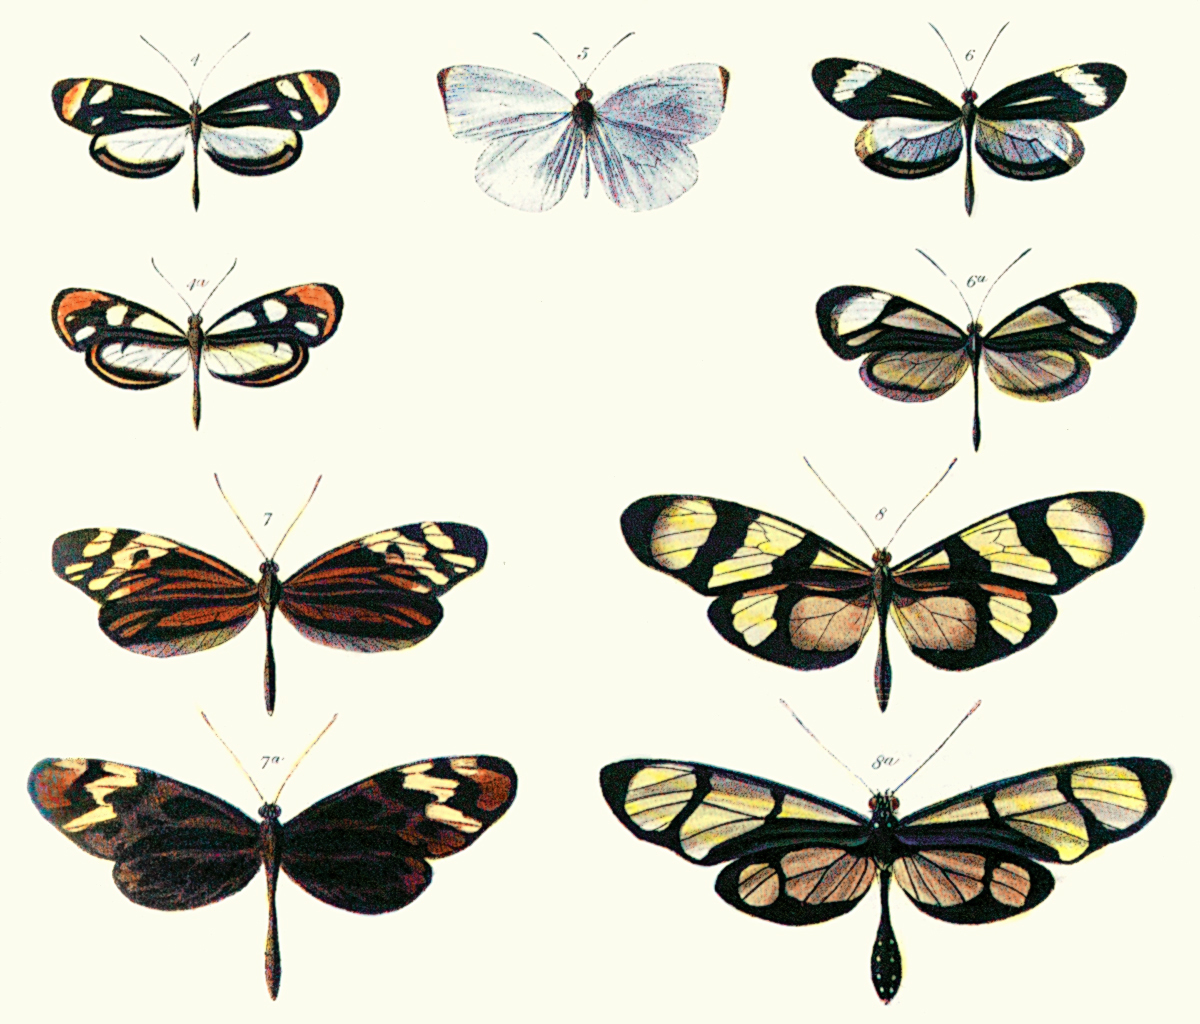
\includegraphics[scale=0.6]{../tex/images/Batesplate_ArM}
		\caption{Plate from Bates (1862) illustrating Batesian mimicry between Dismorphia species (top row, third row) and various Ithomiini (Nymphalidae) (second row, bottom row).}
		\label{fig:batesian-butterfly}
	\end{figure}
}

\frame
{
	\frametitle{Definition of Mimicry}
	\framesubtitle{by Bates and Zoological Congress}
	
	\begin{itemize}
		\item Bates: \textsl{``resemblance in external appearance, shapes and colors between members of widely distinct families."}
		\item International Zoological Congress in Washington, 1963: \textsl{``Mimicry is the close resemblance of one organism to another which, because it is unpalatable and conspicuous, is recognized and avoided by some predators at some times."}
	\end{itemize}
}

\frame
{
	\frametitle{Definition of Mimicry}
	\framesubtitle{by Wallace}
	
	Definition by Wallace and listed in Poulton's \textit{``The color of animals, their meaning and use"}.
		\begin{itemize}
			\item \textsl{``that the imitative species occur in the same area and occupy the same station as the imitated".}
			\item \textsl{``that the imitators are always,"}
				\begin{itemize}
					\item \textsl{``the more defenseless"}
					\item \textsl{``less numerous in individuals"}
					\item \textsl{``differ from the bulk of their allies"}
				\end{itemize}
			\item \textsl{``that the imitation, however minute"}
				\begin{itemize}
					\item \textsl{``is external and visible only"}
					\item \textsl{``never extending to internal characters or to such as do not affect the external appearance."}
				\end{itemize}
		\end{itemize}
}

\subsection{Mullerian Mimicry}

\frame
{
	\frametitle{Mullerian Mimicry}
	
	\begin{itemize}
		\item Two inedible unrelated butterfly species have similar appearance. Bates was unable to explain this.
		\item Explanation came from Fitz Muller in 1878.
		\item Muller's research was in Brazil.
	\end{itemize}

\textbf{Explanation:}
	\begin{itemize}
		\item Predator's limited memory.
		\item Different species loose their number even being inedible.
		\item To save this loss and also for survival of species, inedible ones from different family evolve to have similar appearance.
		\item Phenomenon is referred as Mullerian mimicry, named after Fritz Muller.
	\end{itemize}
}

\frame
{
	\frametitle{Mullerian Mimicry}
	\framesubtitle{Huheey's explanation}
	
	\begin{itemize}
		\item Reduced predation load.
		\item Contribution from naive young predators.
		\item Mutual advertising.
		\item Opportunity from mutation.
		\item Predator's generalization.
	\end{itemize}
	
	\begin{itemize}
		\item Mullerian mimicry is not deception.
		\item Predator's advantage to know all noxious species and deterrent species.
		\item Prey species creating the most traumatic stimuli to a predator have more possibility of the being the model.
	\end{itemize}
}

\frame
{
	\frametitle{Mullerian Mimicry}
	\framesubtitle{Viceroy and Monarch}

	\begin{figure}[H]
		\centering
		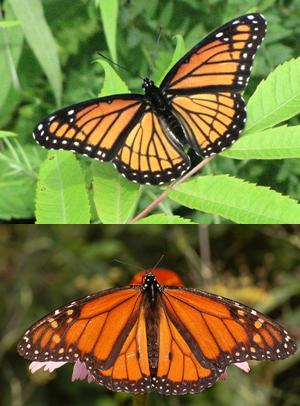
\includegraphics[scale=0.5]{../tex/images/BatesMimButter}
		\caption{A very well-known example of mimicry. Viceroy (top). Unpalatable Monarch (bottom). Image source: \href{http://en.wikipedia.org/wiki/Mullerian_mimicry}{Wikipedia}}
		\label{fig:mullerian-butterfly}
	\end{figure}

}

\subsection{Evolutionary Dynamics}

\frame
{
	\frametitle{Evolutionary Dynamics}
	\framesubtitle{Punctuated Equilibrium}

	Explanation for evolutionary dynamics of mimicry is from Turner. Most sexually reproducing species will remain:
	\begin{itemize}
		\item in extended state of \textit{stasis}.
		\item Little evolutionary change in most of their geological history.
	\end{itemize}
	
	Cladogenesis:
	\begin{itemize}
		\item Process of speciation.
		\item One species split into two distinct species.
		\item It is a discontinuous change, rather than a gradual transformation in a geological time.
	\end{itemize}
}

\frame
{
	\frametitle{Evolutionary Dynamics}
	\framesubtitle{Phyletic Gradualism}

	\begin{itemize}
		\item Species continue to adapt to new environmental and biological selection pressure.
		\item Gradually becomes a new species.
	\end{itemize}
	
	Phyletic gradualism holds that,
	\begin{itemize}
		\item Species population changes gradually.
		\item There is no clear demarcation between an ancestral species and a descendant species.
		\item Gradually changing lineage is divided arbitrarily.
		\item Evolution is 
			\begin{itemize}
				\item smooth
				\item steady
				\item incremental
				\item but not necessary constant and slow rate in geological time scale.
			\end{itemize}
	\end{itemize}
}

\frame
{
	\frametitle{Evolutionary Dynamics}
	\framesubtitle{Punctuated Equilibrium vs. Phyletic Gradualism}

	\begin{figure}[H]
		\centering
		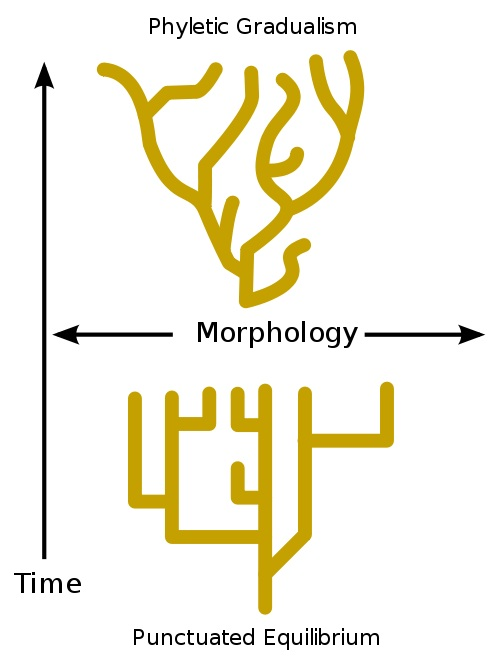
\includegraphics[scale=0.3]{../tex/images/Punctuated-equilibrium}
		\caption{Punctuated equilibrium, bottom, consists of morphological stability and rare bursts of evolutionary change, while the top explains phyletic gradualism. Image source: \href{http://en.wikipedia.org/wiki/Punctuated_equilibrium}{Wikipedia}}
		\label{fig:punctuated-equilibrium}
	\end{figure}
}

\frame
{
	\frametitle{Evolutionary Dynamics}
	\framesubtitle{Turner's Two Stage Model}

	\begin{itemize}
		\item Turner came up with a synthetic theory.
		\item Theory originated from Poulton and Nicholson.
		\item Mimicry arises in two steps:
			\begin{enumerate}
				\item A comparatively large mutation achieves a good approximate resemblance.
				\item A gradual evolutionary change refines the resemblance to a higher degree of perfection.
			\end{enumerate}
		\item This theory has also been applied to Mullerian Mimicry.
	\end{itemize}
}

\subsubsection{Mimicry Ring}

\frame
{
	\frametitle{Mimicry Ring}
	
	\begin{itemize}
		\item Examine the local butterfly fauna in any area of the world to find, between all the aposomatic species, only a limited number of different patterns, normally far smaller than the number of species.
		\item Each cluster of species, all sharing a common pattern is termed as Mullerina mimicry ring.
		\item Consider all the rain forest in South and Central America, most of the long winged butterflies (ithomiids, danaids and heliconids) belong to one of only five different rings.
	\end{itemize}	
}

\frame
{
	\frametitle{Mimicry Ring}
	\framesubtitle{Formation}
	
	Turner's theory of Mimicry Ring Formation, takes into account
	\begin{itemize}
		\item the level of protection of different rings
		\item their difference in phenotypic warning patterns.
	\end{itemize}
	
}

\frame
{
	\frametitle{Mimicry Ring}
	\framesubtitle{Formation}

	Varying these two parameters give different formation of mimicry rings:
	\begin{itemize}
		\item Similar pattern in one habitat:
			\begin{itemize}
				\item Similar enough that the envelop of protection in one provides protection to the other.
				\item \textbf{Result:} Natural protection of mutual convergence.
			\end{itemize}
		\item Very dissimilar patterns:
			\begin{itemize}
				\item Envelop of protection do not overlap. Predator consuming one will not mistake of the other pattern.
				\item \textbf{Result:} No convergence, two patterns will remain distinct.
			\end{itemize}
		\item Mutation:
			\begin{itemize}
				\item Mutation can lead one species into the envelop of protection of another species. 
				\item \textbf{Result:} Gradual convergence of one pattern with another.
			\end{itemize}
	\end{itemize}
}